%
% Descriptions of the various teams.  Volunteering section will refer to this.
%


\chapter{Crew Manifest}
\label{ch:teams}

These are all the teams that support \gls{ttm}.  You can contact these teams or the \gls{ttm} leadership by sending email to \url{connect@tothemoonburn.com}.  Each team also has its own contact email, which is given below.
% * <mcoletti@gmail.com> 2018-05-05T21:21:35.396Z:
% 
% > These are all the teams that support the \gls{ttm}.
% Expand on this.
% 
% ^.

\begin{multicols}{2}
\vbox{
\subsection*{Flight Directors / Event Leads}
The \gls{eventleads} are the acting managers during the event itself.  Through close communication with each Team Lead, they effectively ensure  that all on-site operations run smoothly.  And they drive golf carts.

\begin{description}[leftmargin=6em,noitemsep,style=nextline]
   \item[Leads:] Andrea ``Gem'' Kerns, Gabrielle ``Nectar'' Stewart,
   \item[Co-leads:]  Ben ``Cheesepants'' Bj{\o}st{\aa}d, Willow ``Militits'' Gaia
   \item[Contact:] \url{connect@tothemoonburn.com}
\end{description}
}

\subsection*{ART Team}
The Art Team stays connected with artists from initial inquiry about Art Registration and / or Art Grant Application, communicates with safety teams and BOD about amounts granted, fire and other safety concerns regarding interactive art and about feasibility and scope of art projects. Art Team also works closely with placement to ensure the best spot for any art projects. 

\begin{description}[leftmargin=6em,noitemsep,style=nextline]
   \item[Lead:] Katie ``Creamy'' Miller
   \item[Co-leads:] KT Wiles
   \item[Contact:] \url{artgrants@tothemoonburn.com}
\end{description}


\vbox{
\subsection*{Conclave / Fire Prop Safety}
This team is responsible for the conclave fire spinning event that occurs just before the \gls{effigy} and \gls{temple} burn.

\begin{description}[leftmargin=6em,noitemsep,style=nextline]
   \item[Lead:] Gabrielle ``Nectar'' Stewart
   \item[Co-leads:] Alicia ``Alley Hoops'' Westbrook
   \item[Contact:] \url{conclave@tothemoonburn.com}
\end{description}
}

% This team is responsible for the conclave fire spinning event that occurs just before the \gls{effigy} and \gls{temple} burn.

\subsection*{DPW}
The \gls{dpw} team is responsible for handling the event's logistics, electrical power management, and infrastructure.

\gls{dpw} is looking for \glspl{shiftlead} to cover all of the listed shifts.  Please contact \gls{dpw}  if you are interested in becoming a \gls{shiftlead}.

% I used the addmargin to give this description list a little nudge to 
% prevent confusion for the description lists used for the leads/co-leads
\begin{addmargin}[.3cm]{0cm}
\begin{description}[noitemsep]
% 	\item[DPW:] The team here to take care of the infrastructure, and help keep the wheels on the bus.
	\item[Doozers:] "Do" The Things: Can get things done: lift, tote, dig
	\item[Dispatch:] Organized Soul, Radio trained, likes clipboards - must be approved by \gls{dpw} lead
	\item[Burn Down:] Preps structure for burn down.
\end{description}
\end{addmargin}

\Gls{dpw} meets at \gls{groundcontrol}.

\begin{description}[leftmargin=6em,noitemsep,style=nextline]
   \item[Lead:] Evans Manrique
   \item[Co-leads:] Jack Holloway and Cyrus Nahkjavan
   \item[Contact:] \url{DPW@tothemoonburn.com}
\end{description}

% The \gls{dpw} team is responsible for handling the event's logistics and infrastructure.

\subsection*{Effigy}
This team is responsible for the construction of the main effigy burned on Saturday night.

\begin{description}[leftmargin=6em,noitemsep,style=nextline]
   \item[Lead:] Ezra ``Ezra Everywhere'' Bowers 
   \item[Co-leads:] Josh Boyer
   \item[Contact:] \url{effigy@tothemoonburn.com}
\end{description}

% This team is responsible for the construction of the main effigy burned on Saturday night.

\subsection*{Fire Safety}
This teams helps provide a safe environment for fire art, the \gls{effigy}, and the \gls{temple}. They patrol the burn to help make sure that fire art and fire performance are safely done.

\begin{addmargin}[.3cm]{0cm}
\begin{description}[noitemsep]
	\item[Dirt Patrol:] Looks for fires out of place and ensures that fire spinners are spinning safely.
\end{description}
\end{addmargin}

This year we are combining Fire Safety with \gls{rangers}. If you have experience and would like to be a part of the Fire Safety Team, we need you. Please contact the Fire Safety Lead, Critter, directly to sign-up for these shifts. We are directing everyone to \gls{rangers} shifts. We will have onsite training for Fire Safety and Rangering!

\begin{description}[leftmargin=6em,noitemsep,style=nextline]
   \item[Lead:] Vicki ``Critter'' Coleman
   \item[Co-leads:] James ``Robin Souls'' Raley, Alyshia ``SecoriaDaKitten'' Davis
   \item[Contact:] \url{firesafety@tothemoonburn.com}
\end{description}

% Ensuring that effigy and temple burns are safe is the responsibility of this team.

\subsection*{Gate}
The \gls{gate} team is the first to welcome participants home, takes invites, id's, signed waivers, and records emergency contact info.

This team meets at the \gls{launchpad}.

\begin{description}[leftmargin=6em,noitemsep,style=nextline]
   \item[Lead:] Mandy Kees
   \item[Co-leads:] Caleb Ditchfield
   \item[Contact:] \url{gate@tothemoonburn.com}
\end{description}


\subsection*{Greeters}
% These are the kind and gentle folks that welcome you home.  They will check your tickets, put on your wristbands, and will help orient you on where to go and what to do at \gls{ttm}.  They also make sure that all arriving crew members are aware of and will adhere to the \gls{tenprinciples} and the \gls{eleventhprinciple}.

\paragraph{Who We Are}
We are the brightly shining faces of To The Moon.  We are the ones that will help you blast off into a world of beauty you’ve never know.

\paragraph{What We Do}

As Greeters, we are the first group to welcome astronauts to the Launch Pad, and we absolutely love doing it!  We, along with Gate, make the first impression on this voyage.  We help set expectations and get to communicate with the flight crew for the very first time. 

Our job is to educate ourselves deeply on the meaning of the \gls{tenprinciples} so that we can impart that knowledge onto our participants.  We're also well versed in the \gls{eleventhprinciple} and are happy to discuss!  We are here to clarify any questions you have regarding general operating procedures on the Moon. 

We are passionate about the beautiful land that is Spirit Crossing, and have educated ourselves deeply on the history of the land and special facts that are critical to understand in order to give back to nature the way she gives to us. 

Looking for some sweet \gls{swag}? Look no further than the \gls{greeter} station!  Want a good spanking?  Hey, if you say it's ok, then we're ok with it!  Have questions about where to go to sign up to volunteer? We got it!  Interested in picking up a ``No Photos'' wristband? That's covered, too!  Want to know which camps are kid-friendly?  Done and done!

Greeters are all about having FUN!  Our goal is to get you excited about coming home!  We want everyone to be safe and knowledgeable and have a hell of a time doing it!   

\paragraph{What We Need}

We are looking for outgoing, space-age, creative people to join our band of misfits.  If you are dedicated, patient, have great communication skills, and are ready to take on the truly awesome role of creating out-of-this-world merriment and moon-like magic, then volunteer with us. 

See you on the Moon!!!!

The \glspl{greeter} meet at the \gls{launchpad}.

\begin{description}[leftmargin=6em,noitemsep,style=nextline]
   \item[Lead:] Ashley ``Bones'' Maynard
   \item[Co-leads:] Alicia ``Alley Hoops'' Westbrook
   \item[Contact:] \url{greeters@tothemoonburn.com}
\end{description}

% These are the kind and gentle folks that welcome you home.  They will check your tickets, put on your wristbands, and will help orient you on where to go and what to do at \gls{ttm}.  They also make sure that all arriving crew members are aware of and will adhere to the \gls{tenprinciples} and the \gls{eleventhprinciple}.

\subsection*{\Gls{lamplighters}}
These participants gather before dusk to ceremonially light our moonbase with lanterns, and then gathers them each morning.   
% The \gls{lamplighters} is a burner tradition that started in 1993.  The \gls{lamplighters} are a somber procession starts at twilight each night to kindle torches to help light our way through the night.

Meets at the \gls{cockpit}.

\begin{description}[leftmargin=6em,noitemsep,style=nextline]
   \item[Lead:] Awno Ka
   \item[Co-leads:] Niki Austin and Rebecca JOhnson
   \item[Contact:] \url{lamplighters@tothemoonburn.com}
\end{description}

% The \gls{lamplighters} is a burner tradition that started in 1993.  The \gls{lamplighters} are a somber procession starts at twilight each night to kindle torches to help light our way through the night.


\subsection*{Leave No Trace}
These crew members are responsible for ensuring that the grounds are as we found them --- free of any artifacts of our presence, such as bottle caps, empty bottles, forgotten items, and any other \gls{moop}.

\begin{description}[leftmargin=6em,noitemsep,style=nextline]
   \item[Lead:] Henry ``Jawk'' McElreath
   \item[Co-leads:] Liz ``Freedom''
   \item[Contact:] \url{LNT@tothemoonburn.com}
\end{description}

% These crew members are responsible for ensuring that the grounds are as we found them --- free of any artifacts of our presence, such as bottle caps, empty bottles, forgotten items, and any other \gls{moop}.

\subsection*{Parking / L.O.V.E. / GTFIO}
These crew members are responsible for the efficient and safe landing of all vehicles, and for their orderly and speedy departure.  \Gls{gtfio} is responsible for overall landing and takeoff of vehicles; \gls{love} helps extract vehicles mired on the lunar surface.

\begin{description}[leftmargin=6em,noitemsep,style=nextline]
   \item[Lead:] Kimberly ``Jade'' Lindemann
   \item[Co-leads:] Ian ``Little Buddy'' Brinn
   \item[Contact:] \url{parking@tothemoonburn.com}
\end{description}

% These crew members are responsible for the efficient and safe landing of all vehicles, and for their orderly and speedy departure.  \Gls{gtfio} is responsible for overall landing and takeoff of vehicles; \gls{love} helps extract vehicles mired on the lunar surface.

\subsection*{Perimeter}
% During the \gls{effigy} and \gls{temple} burns, the perimeter crew form a protective barrier to prevent other crew members from participating too intimately with the flames.
These participants meet up before burn time and establish a burn perimeter to aid in the safety of participants during the \gls{effigy} and \gls{temple} burns.

% IMPORTANT INFO FOR ALL PERIMETER VOLUNTEERS! Please read:

% Effigy Outer Perimeter volunteers must meet at the Effigy burn field on Sat, June 16th at 4 PM for training/instructions (EFFIGY burn day). Then meet again at the specific time given at training (around dark-thirty-ish) that same day.

% Temple Outer Perimeter meet at the Effigy burn field on Sat, June 16th at 4 PM for training/instructions (same as EFFIGY perimeter training time), then meet again on SUNDAY, the next day, for Temple burn,  which will burn around 7:30 PM Sunday. So be on field by 7:30 PM.

Perimeter signup only includes \textbf{outer} perimeter shifts (no experience needed other than a mandatory training session (see times above). If you are experienced with perimeter and fire safety and want a shift doing \textbf{inner} perimeter, please email the perimeter lead directly and they will vet you for that.

Meets on the Burn Field

\begin{description}[leftmargin=6em,noitemsep,style=nextline]
   \item[Lead:] Ben ``Cheese Pants'' Bj{\o}st{\aa}d
   \item[Co-leads:] $\emptyset$
   \item[Contact:] \url{perimeter@tothemoonburn.com}
\end{description}

% During the \gls{effigy} and \gls{temple} burns, the perimeter crew form a protective barrier to prevent other crew members from participating too intimately with the flames.

\subsection*{Placement}
This team ensures proper placement of all Theme Camps to avoid sound bleed and bad neighborly relations, creates open camping areas and basically creates the layout of our entire event. Placement works side by side with TCOs and BOD and the end result is our beautiful placement map which you'll find in this survival guide, at the gate and Cockpit. 
\begin{description}[leftmargin=6em,noitemsep,style=nextline]
   \item[Lead:] Brad Tomlinson
   \item[Co-leads:] $\emptyset$
   \item[Contact:] \url{placement@tothemoonburn.com}
\end{description}

% This team assigns locations for theme camps and other temporary emplacements.

\subsection*{Rangers}
% \Gls{rangers} are responsible for keeping the peace.
Rangers are the non-confrontational mediators of community and public safety and providers of information. While on shifts they will carry radios. They are super cool. They stroll the burn and are often the first point of contact should you need assistance.

% I used the addmargin to give this description list a little nudge to 
% prevent confusion for the description lists used for the leads/co-leads
\begin{addmargin}[.3cm]{0cm}
\begin{description}[noitemsep]
	\item[Khaki:] Experienced Ranger running shift, also serves as khaki (dispatch/coordination). Email the Ranger Lead, Runs with Scissors, to sign-up for these shifts.
	\item[Dirt Patrol:] Experienced Ranger, paired with an alpha. For this first burn, both rangers may be inexperienced and if so, will receive on-shift mentoring from lead.
	\item[Alpha:] Inexperienced ranger, paired with a "dirt" ranger. If no dirt ranger available, that's ok. New burn. We will mentor during shift.
\end{description}
\end{addmargin}

Meets at \gls{missioncontrol}.

\begin{description}[leftmargin=6em,noitemsep,style=nextline]
   \item[Lead:] Don ``Runs With Scissors'' Coleman
   \item[Co-leads:] Alan ``Weatherman'' Huskey, Eli ``Fragile Turtle'' Anderson 
   \item[Contact:] \url{rangers@tothemoonburn.com}
\end{description}

% \Gls{rangers} are responsible for keeping the peace.


\subsection*{Survival Guide}
\label{sec:survivalguide}
The \gls{survivalguide} team is responsible for the creation, printing, and distribution of the \gls{preflightmanual} and \gls{survivalguide}. We hope you enjoy this guide and find it helpful!

\begin{description}[leftmargin=6em,noitemsep,style=nextline]
   \item[Lead:] Mark ``Piprrr'' Coletti
   \item[Co-leads:] Andy ``Raptor'' Berres, Ashley ``Bones'' Maynard
   \item[Contact:] \url{survivalguide@tothemoonburn.com}
\end{description}

% The \gls{survivalguide} team is responsible for the creation, printing, and distribution of the \gls{preflightmanual} and \gls{survivalguide}.

\subsection*{Tbase / Sanctuary}

\Gls{tbass} provides a calm, safe space for burners who need a chance to process and integrate their experiences at and responses to the burn. We provide a supportive environment for anyone who needs reassurance, assistance, or just some peace and quiet to work through a current experience or their response to a previous experience. A burn provides a multitude of stimuli, and \gls{tbass}  offers a chance to step back, ground oneself, and experience the transformative process than being home can bring.

Volunteers should be prepared to be sober and unaltered for the duration of a 4-hour shift and able to remain calm when dealing with participants who are distressed, emotional, or experiencing an altered perception of the world around them. Anyone who has previously done Tranquility Base training for Alchemy or Euphoria, Sanctuary training for Ignite!, Transformus, or Flipside, or Zendo Project training for Burning Man can sign up for volunteer shifts now and only needs to attend a brief refresher session and an overview of To The Moon radio protocols (if you have done training for harm reduction/safe space teams at other burns, please contact Mango, the Tranquility Base Team Lead, to discuss your background). If you have not done training, please plan to attend one of the on-site training sessions on Thursday or Friday evening, and you will be able to sign up for volunteer shifts later in the burn at the end of the training or you may sign up for shifts now as long as you attend a training before your shift is scheduled.

Please plan to attend one of the on-site training sessions.

This team meets at \gls{tbass}, of course.

\begin{description}[leftmargin=6em,noitemsep,style=nextline]
   \item[Lead:] Ann ``Mango'' Grens
   \item[Co-leads:] Jo Herrera, Stan Davis
   \item[Contact:] \url{tbase@tothemoonburn.com}
\end{description}

\begin{center}
	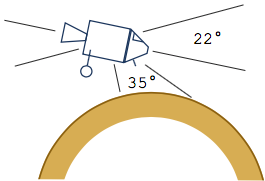
\includegraphics[width=\columnwidth]{images/landing3}
\end{center}

\subsection*{Temple}
This crew assembles and deploys the \gls{temple} to be burned on the last night of \gls{ttm}.

Please note that a few hands are needed to help clean up on Monday after the Temple burn from the night before. Please be sure to pack up your camp before reporting for this shift as the burn will be ended and this shift requires ``late stay'' permission.

\begin{description}[leftmargin=6em,noitemsep,style=nextline]
   \item[Lead:] Michael ``Lunar'' Luber
   \item[Co-leads:] Matthew Horner
   \item[Contact:] \url{temple@tothemoonburn.com}
\end{description}

% This crew assembles and deploys the \gls{temple} to be burned on the last night of \gls{ttm}.
\columnbreak

\subsection*{\acrlong{vc}}
% \Gls{ttm} runs on volunteers, and this stalwart crew makes sure that all the teams have the necessary folks to work effectively.
These volunteers wrangle participants of the burn into needed volunteer positions to keep things running. \glspl{vc} help people check their scheduled shifts as well as sign up for shifts. If you know how sexy volunteering is and want to meet like minded folks, this is a good team for you! We keep volunteers informed of updates during the burn and help teams fulfill unforeseen volunteer needs as they could arise during the burn.

This is also a place for people to come get information about burn happenings, times, locations, and whereabouts to things such as: workshops, theme camps, and events. Sometimes we even help people find themselves!

This team meets at the \gls{cockpit}.

\begin{description}[leftmargin=6em,noitemsep,style=nextline]
   \item[Lead:] Tonya ``Dusty Lashes'' Weisenseel
   \item[Co-leads:] Julie Reach, CeCe ``Platinum'' Hue
   \item[Contact:] \url{volunteer@tothemoonburn.com}
\end{description}

% \Gls{ttm} runs on volunteers, and this stalwart crew makes sure that all the teams have the necessary folks to work effectively.

\end{multicols}

\vspace*{\fill}
\begin{center}
	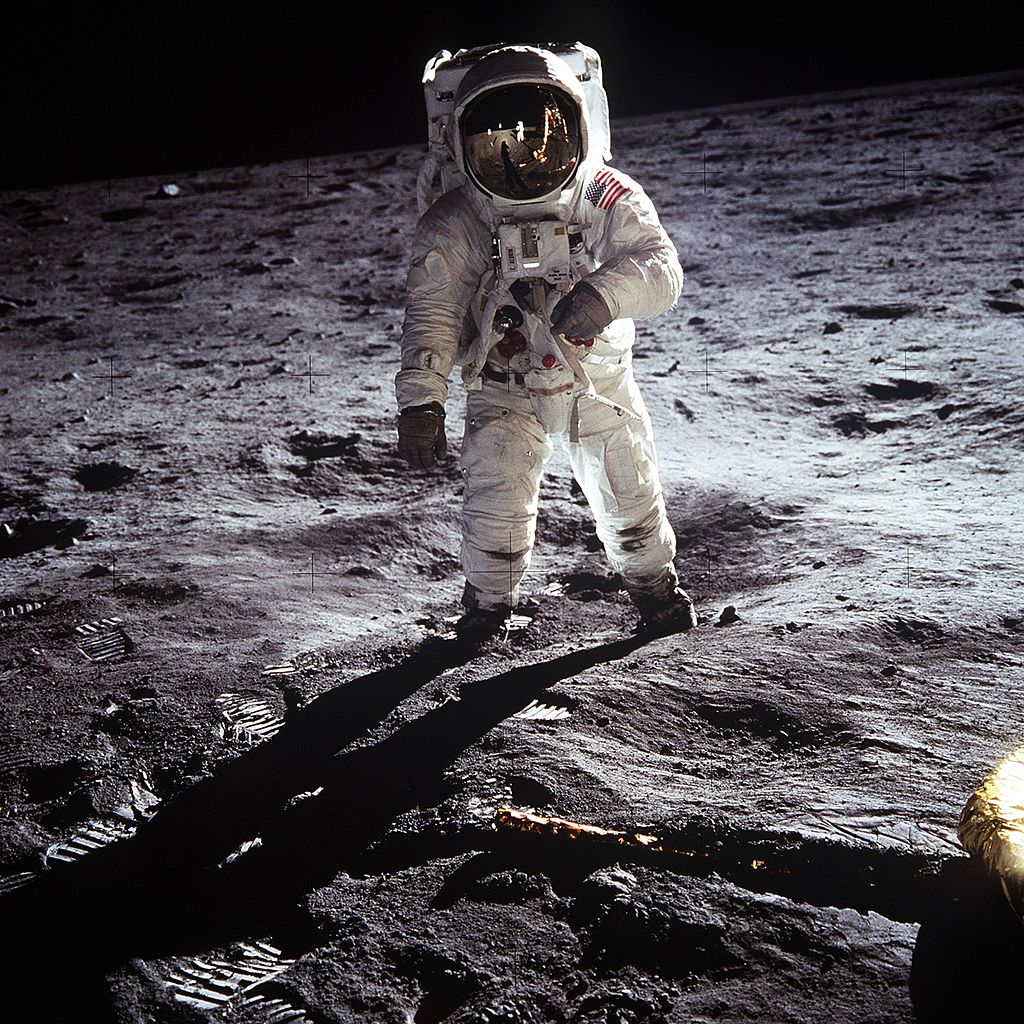
\includegraphics[width=.9\textwidth]{images/Aldrin_Apollo_11}
    \label{image:buzzaldrin}
\end{center}
\vspace*{\fill}



